\documentclass{article}

\usepackage{tikz}

\begin{document}
	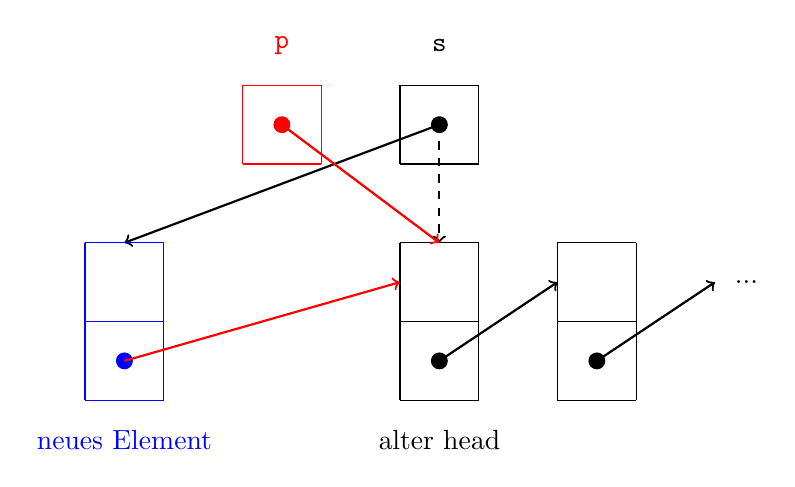
\begin{tikzpicture}
		\draw (0,-1) -- (1,-1);
		\draw (0,-2) -- (1,-2);
		\draw (0,-1) -- (0,-2);
		\draw (1,-1) -- (1,-2);
		\draw[fill=black] (0.5,-1.5) circle (0.1);
		\draw[->, thick, dashed] (0.5,-1.5) -- (0.5,-3);
		\draw[->, thick] (0.5,-1.5) -- (-3.5,-3);
		\node at (0.5,-0.5) (s) {\texttt{s}};
		
		\draw (0,-3) -- (0,-5);
		\draw (0,-3) -- (1,-3);
		\draw (1,-3) -- (1,-5);
		\draw (0,-5) -- (1,-5);
		\draw (0,-4) -- (1,-4);
		\draw[fill=black] (0.5,-4.5) circle (0.1);
		\draw[->, thick] (0.5,-4.5) -- (2,-3.5);
		\node at (0.5,-5.5) (alt) {alter head};
		
		\draw (2,-3) -- (2,-5);
		\draw (2,-3) -- (3,-3);
		\draw (3,-3) -- (3,-5);
		\draw (2,-5) -- (3,-5);
		\draw (2,-4) -- (3,-4);
		\draw[fill=black] (2.5,-4.5) circle (0.1);
		\draw[->, thick] (2.5,-4.5) -- (4,-3.5);
		\node at (4.4,-3.5) (n) {...};
		
		\draw[red] (-2,-1) -- (-1,-1);
		\draw[red] (-2,-2) -- (-1,-2);
		\draw[red] (-2,-1) -- (-2,-2);
		\draw[red] (-1,-1) -- (-1,-2);
		\draw[fill=red, red] (-1.5,-1.5) circle (0.1);
		\draw[->, thick, red] (-1.5,-1.5) -- (0.5,-3);
		\node[red] at (-1.5,-0.5) (s) {\texttt{p}};
		
		\draw[blue] (-4,-3) -- (-3,-3);
		\draw[blue] (-4,-3) -- (-4,-5);
		\draw[blue] (-3,-3) -- (-3,-5);
		\draw[blue] (-4,-4) -- (-3,-4);
		\draw[blue] (-4,-5) -- (-3,-5);
		\draw[fill=blue, blue] (-3.5,-4.5) circle (0.1);
		\draw[->, thick, red] (-3.5,-4.5) -- (0,-3.5);
		\node[blue] at (-3.5,-5.5) (neu) {neues Element};
	\end{tikzpicture}
	
	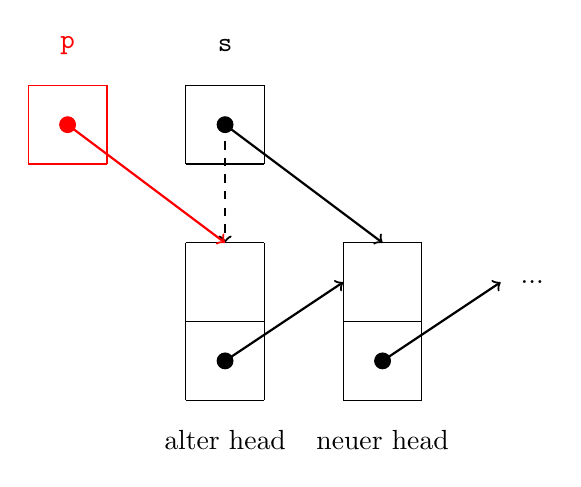
\begin{tikzpicture}
		\draw (0,-1) -- (1,-1);
		\draw (0,-2) -- (1,-2);
		\draw (0,-1) -- (0,-2);
		\draw (1,-1) -- (1,-2);
		\draw[fill=black] (0.5,-1.5) circle (0.1);
		\draw[->, thick, dashed] (0.5,-1.5) -- (0.5,-3);
		\draw[->, thick] (0.5,-1.5) -- (2.5,-3);
		\node at (0.5,-0.5) (s) {\texttt{s}};
		
		\draw (0,-3) -- (0,-5);
		\draw (0,-3) -- (1,-3);
		\draw (1,-3) -- (1,-5);
		\draw (0,-5) -- (1,-5);
		\draw (0,-4) -- (1,-4);
		\draw[fill=black] (0.5,-4.5) circle (0.1);
		\draw[->, thick] (0.5,-4.5) -- (2,-3.5);
		\node at (0.5,-5.5) (alt) {alter head};
		
		\draw (2,-3) -- (2,-5);
		\draw (2,-3) -- (3,-3);
		\draw (3,-3) -- (3,-5);
		\draw (2,-5) -- (3,-5);
		\draw (2,-4) -- (3,-4);
		\draw[fill=black] (2.5,-4.5) circle (0.1);
		\draw[->, thick] (2.5,-4.5) -- (4,-3.5);
		\node at (2.5,-5.5) (neu) {neuer head};
		\node at (4.4,-3.5) (n) {...};
		
		\draw[red] (-2,-1) -- (-1,-1);
		\draw[red] (-2,-2) -- (-1,-2);
		\draw[red] (-2,-1) -- (-2,-2);
		\draw[red] (-1,-1) -- (-1,-2);
		\draw[fill=red, red] (-1.5,-1.5) circle (0.1);
		\draw[->, thick, red] (-1.5,-1.5) -- (0.5,-3);
		\node[red] at (-1.5,-0.5) (s) {\texttt{p}};
	\end{tikzpicture}
\end{document}